\chapter{Source transformations and pitfalls of semantic integrity}
With the information and methodology we have gathered so far, we can now apply actual changes to the target source code. One could think that the 'hard' part is over. And from this on it is mere cause of 'find and replace'. In this section we will deliberately get lost in a chain of changes and surplus changes, before we discover a rather elegant solution. This is to show, how complex this supposedly trivial topic is and how seemingly small changes can imply tremendous impact on the target source code. Without a clean concept of what needs, should and mustn't change the rat tail of code changes will grow.\\\\
First of all we need a second data aggregation step, because without going too far now, there is lots of things that need change and lots of information we need, to do so. For now lets start with something we can change, without any additional information: The new struct for the cold fields.\\
For a record \textit{Foo} definition like the one in line 1 to 7 of \refcode{example_split_0} we could create a struct containing the cold fields and call it \textit{coop\_cold\_fields\_Foo}. The name is quite arbitrary but includes \textit{'coop'} and is expressive so further investigation and troubleshooting is not complicated unnecessarily. Also this attenuates the chance of accidentally running into namespace conflicts. This convention is applied to most changes, however to reduce the excerpts' sizes we will use shortened, yet expressive abbreviations.\\
The newly created \textit{cold\_struct} holds the cold fields. The original record keeps the hot fields. It is also given an additional public section for upcoming additions, like a pointer to an instance of the cold struct. To ensure that resources are cleaned up properly we will also create a destructor in the original record (\refcode{example_split_0} line 26) that on the one hand destroys the cold\_struct instance and also notices the free list, that the instance's space is now reusable.
\begin{lstlisting}[language=C++,name={Example of how a record will be split.},label={example_split_0}]
struct Foo {
	int hot_0;
	int hot_1;
	int cold_0 = 10;
	int cold_1;
	int cold_2
};

void bar(Foo *f){f->cold_1 = 100;}

//becomes:
struct cold_struct {
	int cold_0 = 10;
	int cold_1;
	int cold_2
};
struct Foo {
	int hot_0;
	int hot_1;
	
	Foo(){
		cold_data_ptr = 
			new (cold_free_list.get<cold_struct>()) cold_struct();
	}
	
	~Foo(){
		cold_data_ptr->~cold_struct();
		cold_free_list.free(cold_data_ptr);
	}
public:
	cold_struct *cold_data_ptr;

};

void bar(Foo *f){f->Foo::cold_data_ptr->cold_1 = 100;}
\end{lstlisting}
Extracting the cold fields implies changes to several parts of the target program so to further adapt it to the new data layout we will need to gather the AST nodes for several constructors and operators of the original record definition, the destructor, member expressions associating cold fields, calls of the new operator as well ad delete calls associating cold field and access spec declarations (to ensure code injections are placed with proper encapsulation).\\
Some AST nodes like constructors and operators can usually be extracted out of the record definition's AST node, however this does not always work properly, especially when the actual definition of the wanted e.g. destructor is in another file. So we need to again traverse the ASTs searching for new information. Luckily this is again rather easy, as we can use the AST Matchers \refcodep{second_data_aggregation}.
\begin{lstlisting}[language=C++, name={Shortened excerpts for some AST Matchers to retreive information we need to implement changes - second data aggregation.}, label={second_data_aggregation}]
//find access specs:
cxxRecordDecl(hasDescendant(accessSpecDecl().bind(coop_access_s)))
//find delete calls
cxxDestructorDecl(isDefinition(), hasName(regex))
//find constructor definitions
cxxConstructorDecl(isDefinition(), unless(isImplicit()))
//find copy assignment operator
cxxMethodDecl(isDefinition(), isCopyAssignmentOperator(), unless(isImplicit()))
//find move assignment operator
cxxMethodDecl(isDefinition(), isMoveAssignmentOperator(), unless(isImplicit()))
\end{lstlisting}
\subsection{Redirecting cold field access to the externalized subset}
In line 9 of \refcode{example_split_0} we see a function, that uses a member expression \textit{f->cold\_1} to assign the field \textit{cold\_1} a new value 100. The Expression is now broken after the externalization and needs to be fixed. With the prior AST Matchers we will find every member expression that associates cold data. COOP iterates them and redirects them appropriately. This is rather simple, since all there is to do is injecting access on the cold data pointer first. After retrieving the respective AST node we will assemble the code fragments, we need to constitute the correct access to the cold field.\\
\begin{lstlisting}[language=C++, name={Assembling the proper access ot a cold field through the additional indirection.}, label={redirect_assembly}, morekeywords={stringstream, std}]
std::stringstream access_redirection;
access_redirection << field->getParent()->getQualifiedNameAsString() << "::";
access_redirection << "->" << field_decl_name;
replace_text(mem_expr->getMemberLoc(), access_redirection.str());
\end{lstlisting}
One might notice, that \refcode{redirect_assembly} will produce qualified accesses. Usually COOP will use the record's qualifiers in the target code, to ensure proper namespace associations, but not in this case. Records might happen to be in a sub/super class relation. Whenever a super class and its extension are both splitted (TODO REF SEC inheritance meeh) we need to ensure, that the right cold field struct is accessed.\\
This could either be solved by making the splitted record's name part of it's cold data pointer's identifier (e.g. \textit{cold\_data\_ptr\_Foo} instead of \textit{cold\_data\_ptr}) or by making sure the cold fields original record's allegiance is expressed by qualified access (e.g. \textit{Foo::cold\_field} instead of \textit{cold\_field}).\\\\
Another small but important detail here is, that the original code is replaced from (including) the first character of the fields identifier (\refcode{redirect_assembly} line 4). This way we don't need to even be aware whether or not the original access comes from an instance or a pointer. The access on the cold field will always be through the cold data pointer so we can safely rely on the arrow operator \textit{->} to retrieve it.

\subsection{Guaranteed existence of cold fields }
Access on the cold fields can be redirected to the \textit{cold\_data\_ptr} so the proper field can be dereferenced. But right now we can not guarantee, that whenever the target program expects a cold field to exist, that it actually does.\\
During development redirecting access to a cold field was tested through an inlined access method. This seems like a good practice, since prior to the field access we can check the address for validity and this effectively enables lazy evaluation for the cold fields instantiation. This also meant, that there needed to be several versions of access methods, because different access situations based on const qualifiers would produce compile time errors otherwise. Clang enables us to adjust to those situations. For example a Member Expression's qualified type can easily be accessed through the AST node like this:
\begin{lstlisting}[language=C++, numbers=none, name={Retreiving type information from a clang::MemExpr pointer.}]
	bool is_const = mem_expr->getType().isConstQualified();
\end{lstlisting}
So depending on the qualified types of the member expressions we could decide which access method would not break the code. However as we discussed before, cold fields are not automatically used rarely, they just happen to be used relatively low frequent in comparison to the hot fields. Lazy evaluation and constant additional validation checks could in those cases hurt the runtime instead of initial loads since the original code might access the fields one by one several times. So instead the simple solution is: making the cold data pointer public and letting the target code 'directly' access the pointer to the cold fields. However this also implies that we need another mechanism to ensure, that cold fields are existent/initialized correctly whenever the target program assumed they would be.\\\\
The previous attempt of always accessing cold fields would create an instance of the cold data struct on the spot. Now that we have decided against it and in favor of initial loads we will turn to the original record's constructors. So instead of generating a cold struct instance on demand, we will make sure to create it, when the original record's instance is created. A convenient way to intercept the original record's creation is altering its constructors.\\
That is why we defined AST Matchers to find them. Again retrieving them through the record definition's AST node should work in most cases, but prove to sometimes refer to the constructor's declaration instead of it's definition. There is a few things to be aware of. First of all there can be numerous constructors for a record. In order to guarantee a cold struct instance to be present (and initialized) on creation, we should probably inject the respective line into each constructor. This would certainly work, however is wasteful since there might be delegating constructors. Whenever a constructor merely extends another constructor both of them are executed.\\\\
Fortunately Clang accommodates us with this issue as well. A record's constructors are defined in their own type of AST node called \textit{clang::CXXConstructorDecl}. These nodes know about delegating constructors and let us traverse their call hierarchy easily. So in order to never repeatedly and unnecessarily create a cold struct instance we will follow the constructor's target constructor until we find a 'root constructor' \refcodep{delegating_ctors}.
\begin{lstlisting}[language=C++, name={Traversing the constructors' delegating constructors until we find a 'root' node.}, label={delegating_ctors}, morekeywords={clang, CXXConstructorDecl}]
	clang::CXXConstructorDecl *ctor = ...;
	while(ctor->isDelegatingConstructor())
		ctor = ctor->getTargetConstructor();
\end{lstlisting}
Several constructors might eventually lead to the same root constructors, so besides we also need to refrain from injecting the creation code multiple times to the same constructor now.\\\\
However what do we do if there is no constructor definition at all? Well there will be a constructor but it might be an implicitly generated default constructor. In this case COOP would now actually have to create a 'user-defined' constructor and inject it into the record definition. The actual greatest benefit of the previously mentioned access method is, that we do not rely on altering constructors but can always expect the target code to be in possession of a cold struct instance when needed. Without it we are forced to inject additional constructors. And its getting worse.

\subsection{Semantic integrity and deep copy emulation}
The clear upside of a getter access method that creates cold struct instances on the spot is, that it will never try to dereference a nullpointer due to nonexistent cold data. That is as long as we have enough space reserved in our pool allocator. Same goes for constructor adaptations/creations.\\
At this point COOP faces a major problem. Both of the above attempts do not consider yet, that externalizing the data layout will very directly affect the data flow of the program even after redirecting cold field accesses correctly. The problem is that externalizing a subset of fields will not only affect the code, that is written by the original programmer, but also all of the implicitly generated code, that is yet to come from the compiler.\\
For example for the purpose of testing COOP a program was written that implemented a simple particle system in a classic object oriented manner.
\begin{figure}[ht]
	\begin{minipage}[b]{0.5\linewidth}
		\centering
		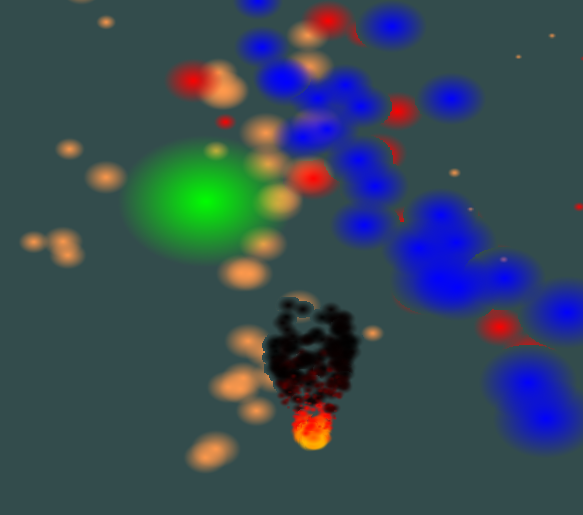
\includegraphics[width=\textwidth,height=.7\textwidth]{PICs/particles}
	\end{minipage}
	\hspace{0.5cm}
	\begin{minipage}[b]{0.5\linewidth}
		\centering
		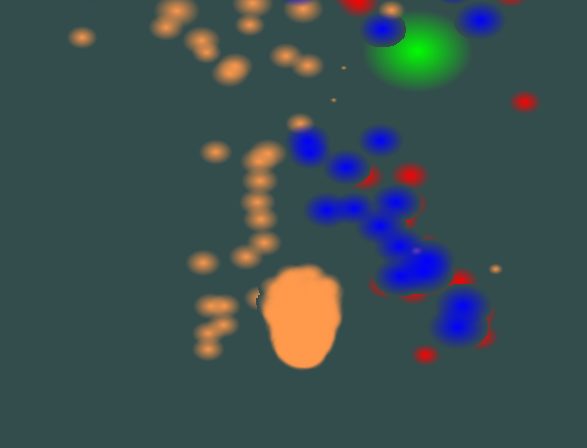
\includegraphics[width=\textwidth,height=.7\textwidth]{PICs/particles_faulty}
	\end{minipage}
\caption{Screenshots of simple particle application. Left - original. Right - faulty shaders on the fire cause of semantic corruption.}\label{particles_faulty}
\end{figure}
\reffig{particles_faulty} shows two screenshots of that application. On the left there are some particles flying around, in their midst burns a cozy particle fire. On the right we see the same application after an early version of coop tried to improve it. We can see, that the particle fire now has another color.\\
To be specific, the particle fire has now another shader. How so? The particle systems defined in the application are initialized with a single particle as their prototype. The fire and the particle gun shooting orange balls share a prototype. The prototype is only changed before it is given to the other particle system as a reference. Since our particles are defined as classic objects, they (amongst others) define their shader as a direct property of theirs. COOP recognized the shader as field that is used rarely compared to the positional traits, as well as the particles velocity, acceleration and mass, that are all used in physics calculations. Consequently the shader field was externalized into a cold struct. When the prototype particle was created for the cozy fire its shader field was initialized with the 'fire shader'. Forth going we created another prototype for the orange particle gun by copying the fire's prototype. We then altered the new prototype copy to make it fit for the particle system shooting orange balls and gave it the 'orange shader'. This is the part where we accidentally messed up the fire particle system's prototype.\\
By externalizing the cold subset from the particle record, we not only affected the fields direct associations, but also the programs interactions concerning the whole record. Copying the particle record used to copy every single field inside the particle. Where once was (amongst others) the shader field we now copied the pointer to the first prototypes cold data. We have effectively disabled copying of cold data  and created shared state among copied instances of hot data. This is not a semantic equivalent to the original program.\\\\
Actually this outcome can be considered lucky. The consequences of losing semantic integrity can easily break the code. If we were to create temporary copies of our particle, as soon as the copy left the scope it would now destroy the cold struct instance, while the original still depends on it. A quick and dirty fix to this is to make the cold data pointer a shared pointer. This will on the one hand prevent temporary copies to prematurely destroy the shared data, but on the other hand this is still not better. Temporary copies need to be able to alter the copied data, without affecting the original data. The substantial problem here is, that what used to be distinct data is now shared state.\\\\ 
To fix this we now need to make sure, that the copy constructors and/or copy assignment operators work properly after a split, too. Thats why we previously searched for their AST nodes to be able to access and alter their definitions. Also from this point on the house of cards will start to totter. There are several things, we need to consider. Are there any user defined copy constructors/copy assignment operators, because the user will not have included our cold data pointer in the self made copy assignment operator and field access redirection will do the rest.\\
On the other hand when there is no user defined copy assignment operator but an implicit one, we now need to actually make sure, that this copy assignment operator will copy anything but our cold data pointer. On top of that it will need to manually copy all the cold fields. Since it is an assignment both our above methods (access method, constructor initializing) will already have provided us with an instance of the cold data struct, so no need to create a new one.\\
This means iterating all the fields and copying them manually. In case we are dealing with static array types, we will resort to \textit{memcpy}, by determining its size like in \refcode{memcpy_quant}.
\begin{lstlisting}[language=C++, name={Retrieving the size of a static array type through its AST node.}, label={memcpy_quant}]
	siez_t size = field->getASTContext().
		getTypeSizeInChars(dyn_cast_or_null<ConstantArrayType>(type.getTypePtr())).
		getQuantity();
\end{lstlisting}
When there is no user defined copy constructor but an implicit defined one, we also need to do the same for the copy constructor, with the exception, that in this case we also need to generate a new cold struct instance. At least the copy constructor may just use the copy assignment operator. However we have now already bloated the original record definition.\\
Note also, that this is the reason why we can't have the access getter method for that creates cold struct instances on the spot without validation and redundancy checks. While this would work for copy constructors, each time we made use of the copy assignment operator (where we access cold fields) we would create a new instance, even though the assignment determines, that there already is an instance to work with.\\
On top of that since we might have now manually defined a copy constructor/assignment operator, we gave up implicitly defined move semantics for our target program. E.g. a move constructor will be defined implicitly if the respective record does not have a user defined copy constructor/assignment operator \mcp{bjarne_move}{5} (among other criteria). We initially had no problem with move assignment operators and move constructors, since they could just take the pointer to the cold struct instance without a problem.\\
At this point several algorithms might no longer profit from move semantics and instead have to rely on copying which means unnecessary much object creations/deletions. We might have just deteriorated the target programs performance instead of optimizing it. While manually assembling the copy assignment operator was quite possible we can't do the same for the move semantic pendants. We don't know how to destroy the fields on our own and can't just blindly call delete on fields.\\
Luckily if move assignment operators and move constructors were originally implicitly defined and we prevented them with 'user defined' copy constructors/assignment operators, we can bring them back by defining them as \textit{default}.\\\\
At this point we have a working implementation, however there is a solution that requires much less injected code, AST traversal for additional information like constructors/destructors/operators and almost works out of the box.\\
By directly initializing the cold data pointer \textit{in-class} we also affect each constructor. As soon as an instance is initialized it is ensured to point to an instance of a cold data struct. Ironically even though this drastically reduces the required code injections, it also is not yet a semantic equivalent to the original code, because it still suffers from faulty instance copying.\\
Before we mentioned the shared pointer as a quick and dirty 'fix'. Indeed a smart pointer could solve our problems. COOP's solution to maintain semantic integrity with the original program is to emulate a deep copy by defining the behavior in a container for our cold data pointer \refcodep{deep_cpy_ptr}. The important lines are line 8 and 12. In line 12 we make sure, that an instance is created as soon as we create an instance of the hot data (Accordingly the hot data holds an instance of a \textit{deep\_cpy\_ptr}). Line 8 ensures, that when there is a copy, we will copy the actual cold data, rather than only the pointer. 
\begin{lstlisting}[language=C++, name={Shortened version of COOP's container for the pointer to the cold data struct intance. It only defines a single field (the pointer) so no additional memory space is spend.}, label={deep_cpy_ptr}]
	struct deep_cpy_ptr{
		deep_cpy_ptr(){}
		deep_cpy_ptr(const deep_cpy_ptr &other){
			*this=other;
		}
		deep_cpy_ptr & operator=(const deep_cpy_ptr &other){
			if(this==&other)return *this;
			*ptr = *other.ptr;
			return *this;
		}
		~deep_cpy_ptr(){
			ptr->~cold_struct();
			cold_free_list.free(ptr);
		}
		
		cold_struct *ptr = new (cold_free_list.get<cold_struct>()) cold_struct();
	};
\end{lstlisting}
This works fine as the in-class initialization guarantees, that copy construction will create a new cold struct instance and copy assignment will not instantiate redundant cold struct instances.\\
The only thing worth mentioning is, that no matter where a hot data instance is created (be it on the stack or heap), from now on they will each have their own cold struct instance. Our pool allocator for the hot data will provide space for single instance allocations of hot data, however temporary copies of hot data instances on the stack or array allocations on the heap of hot data instances will always create cold struct instances on the pool allocator for cold data. When assigning char arrays to our allocators for them to administrate, we will want to make sure, that there is enough space for the cold data.

\subsection{Constructor initializers associating externalized fields and const qualified cold fields}
Unfortunately under a certain circumstance we can't avoid interfering with constructor definitions. Redirecting cold field associations will implicitly care about cold field initializations happening inside a hot record's constructor. The initialization of cold fields might however also happen through constructor initializers in a member initialization list \refcodep{ctor_initializers}.
\begin{lstlisting}[language=C++, name={Simplified source transformations for problematic cold field initializations in initialization list.}, label={ctor_initializers}]
	struct Foo {
		Foo(int h, float c):hot_field(h), cold_field(c){}
	
		int hot_field;
		float cold_field;
	};
	
	//becomes:
	srtuct cold_data {
		float cold_field;
	};
	struct Foo {
		Foo(int h, float c):hot_field(h){
			cold_data_ptr.ptr->cold_field = c;
		}
	
		int hot_field;
		deep_cpy_ptr cold_data_ptr = ...;
		...
	};
\end{lstlisting}
In this case the cold fields initialization can't remain in the initializer list, because after the split the constructor can't access them the same way. Unfortunately this implies possibly worsened performance, as usually member initialization list can e.g. resort to copy construction directly instead of cunstruction, assignment operator and destruction steps for constructor arguments that are \textit{passed by value}.\\
In order to make the changed source code even compile, COOP will move the cold field initializations into the constructor's body (line 14).\\
However this implies further changes. Whenever a record's constructor initializes non-static cosnt qualified data members, moving their initialization into the constructors body will also result in compilation errors, as they may only be initialized in-class or in member initialization lists.\\
On solution in this case would be to extend the cold struct by an additional constructor, that resemble the target constructor of the hot data record. This way the 'hot constructor' could internally construct the cold struct instance with the appropriate 'cold constructor'. This not only requires us to again bloat the target source code, but also won't work properly considering, that we want to in-class initialize the cold fields instance. Calling an additional 'cold constructor' inside the 'hot constructor' would either lead to multiple cold struct instances per hot instance, or imply a possible costly copy assignment, when all we want to do is modify distinct cold fields.\\\\
Since COOP is meant to be a finalization step  optimization rather than being an iteration based development tool it will simply get rid of the cold field's const qualifier at all.\\
As the const qualifier is merely a developer's guide at the point of COOP's invokation we will want to ignore it in favor of possible performance hazards. So whenever a cold field possesses local const qualifiers, its image in the cold struct will lose local const qualifiers at all.
